\documentclass[tikz,border=2pt]{standalone}
\usepackage{tikz}
\usetikzlibrary{positioning, arrows.meta, calc}
\usepackage{xcolor}

%% Color palette (Tol colourblind-safe, matching existing figures)
\definecolor{research}{HTML}{0077BB}
\definecolor{policy}{HTML}{EE7733}
\definecolor{reference}{HTML}{228833}
\definecolor{sharedbg}{HTML}{444444}

\tikzset{
  base/.style={draw, rounded corners=3pt, align=center,
               inner xsep=6pt, inner ysep=5pt, line width=0.5pt},
  t1/.style={base, fill=reference!12, draw=reference, text width=3.8cm},
  t2/.style={base, fill=research!12, draw=research, text width=3.8cm},
  t3/.style={base, fill=policy!12, draw=policy, text width=3.8cm},
  shared/.style={base, fill=sharedbg!6, draw=sharedbg, text width=13cm},
  arrow/.style={-{Stealth[length=2mm]}, draw=gray!70, line width=0.5pt},
  legbox/.style={draw, rectangle, rounded corners=2pt,
                 minimum width=7mm, minimum height=4mm, inner sep=2pt, line width=0.4pt},
}

\begin{document}
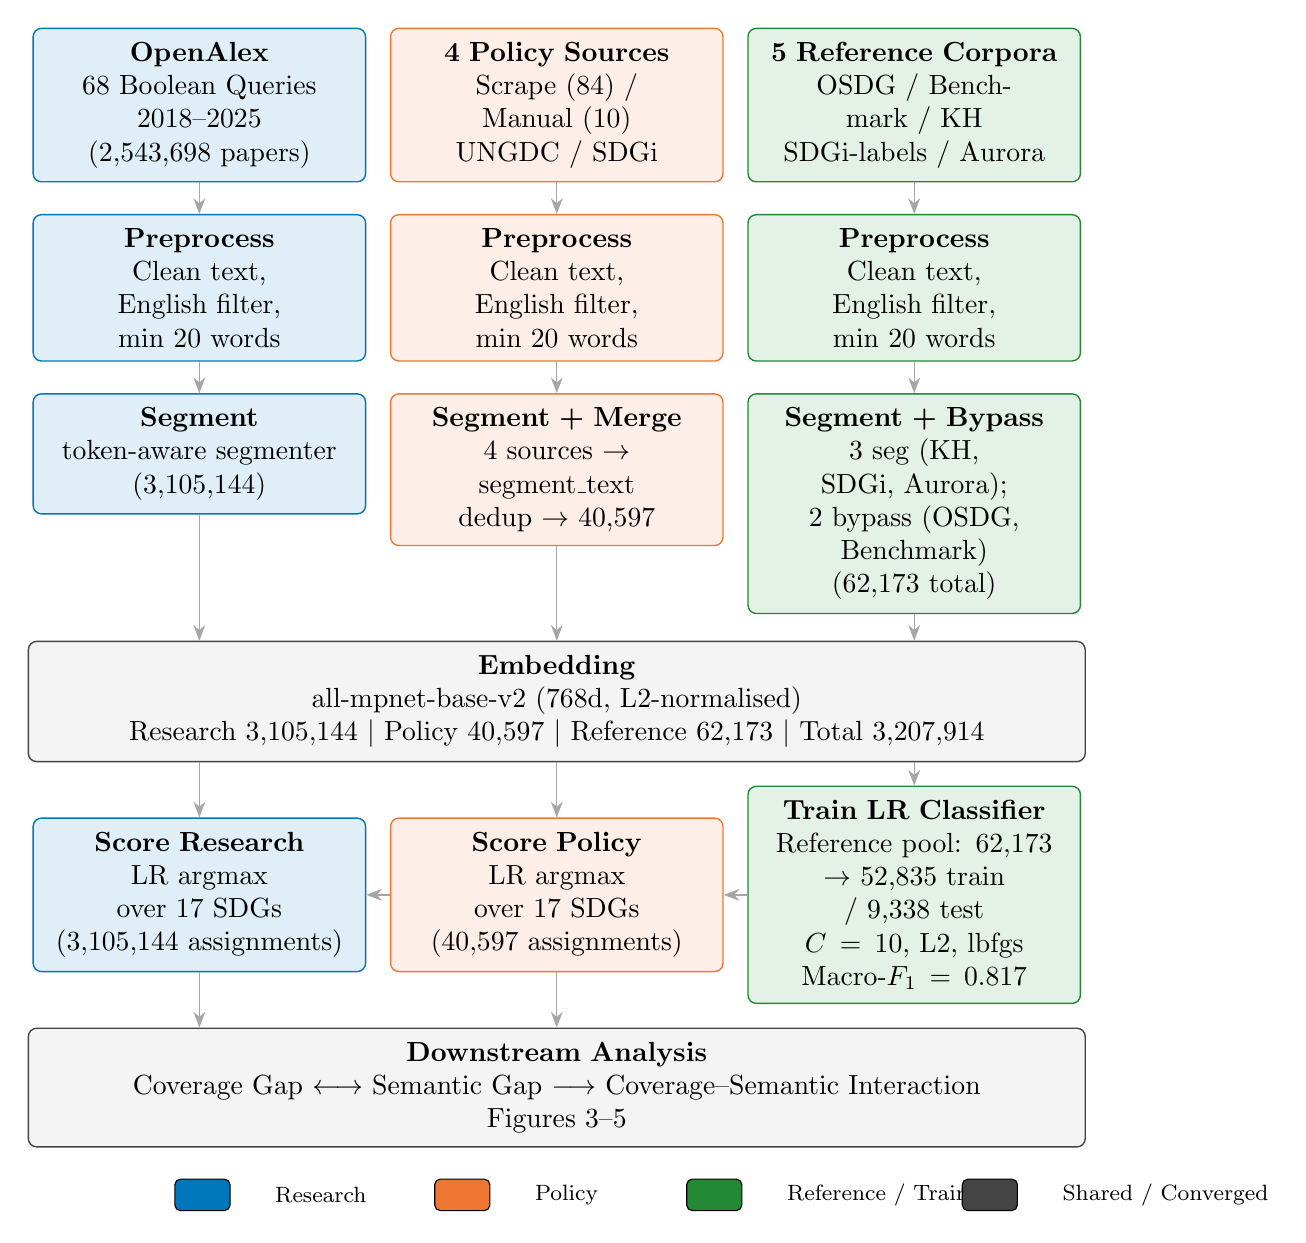
\begin{tikzpicture}[node distance=0.4cm and 0.3cm]

%% ====================  ROW 1: FETCH / SOURCES  ====================

\node[t2] (r_src) {\textbf{OpenAlex}\\68 Boolean Queries\\2018--2025\\(2,543,698 papers)};
\node[t3, right=of r_src] (p_src) {\textbf{4 Policy Sources}\\Scrape (84) / Manual (10)\\UNGDC / SDGi};
\node[t1, right=of p_src] (ref_src) {\textbf{5 Reference Corpora}\\OSDG / Benchmark / KH\\SDGi-labels / Aurora};

%% ====================  ROW 2: PREPROCESS  ====================

\node[t2, below=of r_src] (r_prep) {\textbf{Preprocess}\\Clean text, English filter,\\min 20 words};
\node[t3, below=of p_src] (p_prep) {\textbf{Preprocess}\\Clean text, English filter,\\min 20 words};
\node[t1, below=of ref_src] (ref_prep) {\textbf{Preprocess}\\Clean text, English filter,\\min 20 words};

%% ====================  ROW 3: SEGMENT  ====================

\node[t2, below=of r_prep] (r_seg) {\textbf{Segment}\\token-aware segmenter\\(3,105,144)};
\node[t3, below=of p_prep] (p_seg) {\textbf{Segment + Merge}\\4 sources $\rightarrow$ segment\_text\\dedup $\rightarrow$ 40,597};
\node[t1, below=of ref_prep] (ref_seg) {\textbf{Segment + Bypass}\\3 seg (KH, SDGi, Aurora);\\2 bypass (OSDG, Benchmark)\\(62,173 total)};

%% ====================  ROW 4: EMBED  ====================

\node[shared, below=1.2cm of p_seg] (embed)
  {\textbf{Embedding}\\all-mpnet-base-v2 (768d, L2-normalised)\\
   \textnormal{Research 3,105,144 $\mid$ Policy 40,597 $\mid$ Reference 62,173 $\mid$ Total 3,207,914}};

%% ====================  ROW 5: TRAIN + SCORE  ====================

\node[t2, below=0.7cm of embed.south -| r_seg.south] (score_res)
  {\textbf{Score Research}\\LR argmax over 17 SDGs\\(3,105,144 assignments)};

\node[t3, right=0.3cm of score_res] (score_pol)
  {\textbf{Score Policy}\\LR argmax over 17 SDGs\\(40,597 assignments)};

\node[t1, right=0.3cm of score_pol] (train)
  {\textbf{Train LR Classifier}\\Reference pool: 62,173\\
   $\rightarrow$ 52,835 train / 9,338 test\\
   $C=10$, L2, lbfgs\\
   Macro-$F_1 = 0.817$};

%% ====================  ROW 6: ANALYSIS  ====================

\node[shared, below=0.5cm of $(score_res.south)!0.5!(train.south)$] (analysis)
  {\textbf{Downstream Analysis}\\Coverage Gap $\longleftrightarrow$ Semantic Gap $\longrightarrow$ Coverage--Semantic Interaction\\Figures 3--5};

%% ====================  ARROWS  ====================

%% Research track
\draw[arrow] (r_src)    -- (r_prep);
\draw[arrow] (r_prep)   -- (r_seg);
\draw[arrow] (r_seg)    -- (r_seg |- embed.north);
\draw[arrow] (embed.south -| score_res.north) -- (score_res.north);

%% Policy track
\draw[arrow] (p_src)    -- (p_prep);
\draw[arrow] (p_prep)   -- (p_seg);
\draw[arrow] (p_seg)    -- (embed.north);
\draw[arrow] (embed.south -| score_pol.north) -- (score_pol.north);

%% Reference track
\draw[arrow] (ref_src)  -- (ref_prep);
\draw[arrow] (ref_prep) -- (ref_seg);
\draw[arrow] (ref_seg)  -- (ref_seg |- embed.north);
\draw[arrow] (embed.south -| train.north) -- (train.north);

%% Model from Train to Score
\draw[arrow] (train.west) -- (score_pol.east);
\draw[arrow] (score_pol.west) -- (score_res.east);

%% Score → Analysis
\draw[arrow] (score_res) -- (score_res |- analysis.north);
\draw[arrow] (score_pol) -- (score_pol |- analysis.north);

%% ====================  LEGEND  ====================

\coordinate (leg) at ($(analysis.south) - (0,0.6)$);

\node[legbox, fill=research]  at ([xshift=-4.5cm]leg) {};
\node[font=\footnotesize, anchor=west] at ([xshift=-3.7cm]leg) {Research};

\node[legbox, fill=policy]    at ([xshift=-1.2cm]leg) {};
\node[font=\footnotesize, anchor=west] at ([xshift=-0.4cm]leg) {Policy};

\node[legbox, fill=reference] at ([xshift=2.0cm]leg) {};
\node[font=\footnotesize, anchor=west] at ([xshift=2.8cm]leg) {Reference / Training};

\node[legbox, fill=sharedbg]  at ([xshift=5.5cm]leg) {};
\node[font=\footnotesize, anchor=west] at ([xshift=6.3cm]leg) {Shared / Converged};

\end{tikzpicture}
\end{document}
